\section{Theorie}
\label{sec:Theorie}

Magnetische Felder werden von elektrischen Strömen und magnetischen Dipolen erzeugt.
Die Grundlage der Berechnung einer magnetischen Flussdichte $\symbf{B}$
am Ort $\symbf{r}$ durch einen stationären elektrischen Strom $I$ ist
das Biot-Savartsche Gesetz
\begin{equation}
  \symbf{B}(\symbf{r}) = \frac{\mu_0}{4 \symup{\pi}}
    \int_C \frac{I \symup{d} \symbf{s} \times \symbf{r}}{r^3}\,.
  \label{eqn:biotsavart}
\end{equation}
Dies ist ein Kurvenintegral über die stromdurchflossene Kurve $C$ mit ihrem
Wegelement $\symup{d}\symbf{s}$. Die magnetische Permeabilität des Vakuums $\mu_0$
hat den definierten Wert $\SI{4\pi e-7}{\henry\per\meter}$.

Eine Spule besteht aus einem gewickelten Draht, der auf einer Basis, meist einem Zylinder mit dem Radius $R$,
aufgebracht ist. Die Windungszahl $n$ drückt die Anzahl der Umläufe des Drahtes aus.
Eine von einem Strom $I$ durchflossene Spule erzeugt ein zur Stromstärke proportionales Magnetfeld.
Eine Skizze dazu ist in Abbildung \ref{fig:spule} zu sehen.

\begin{figure}
  \centering
  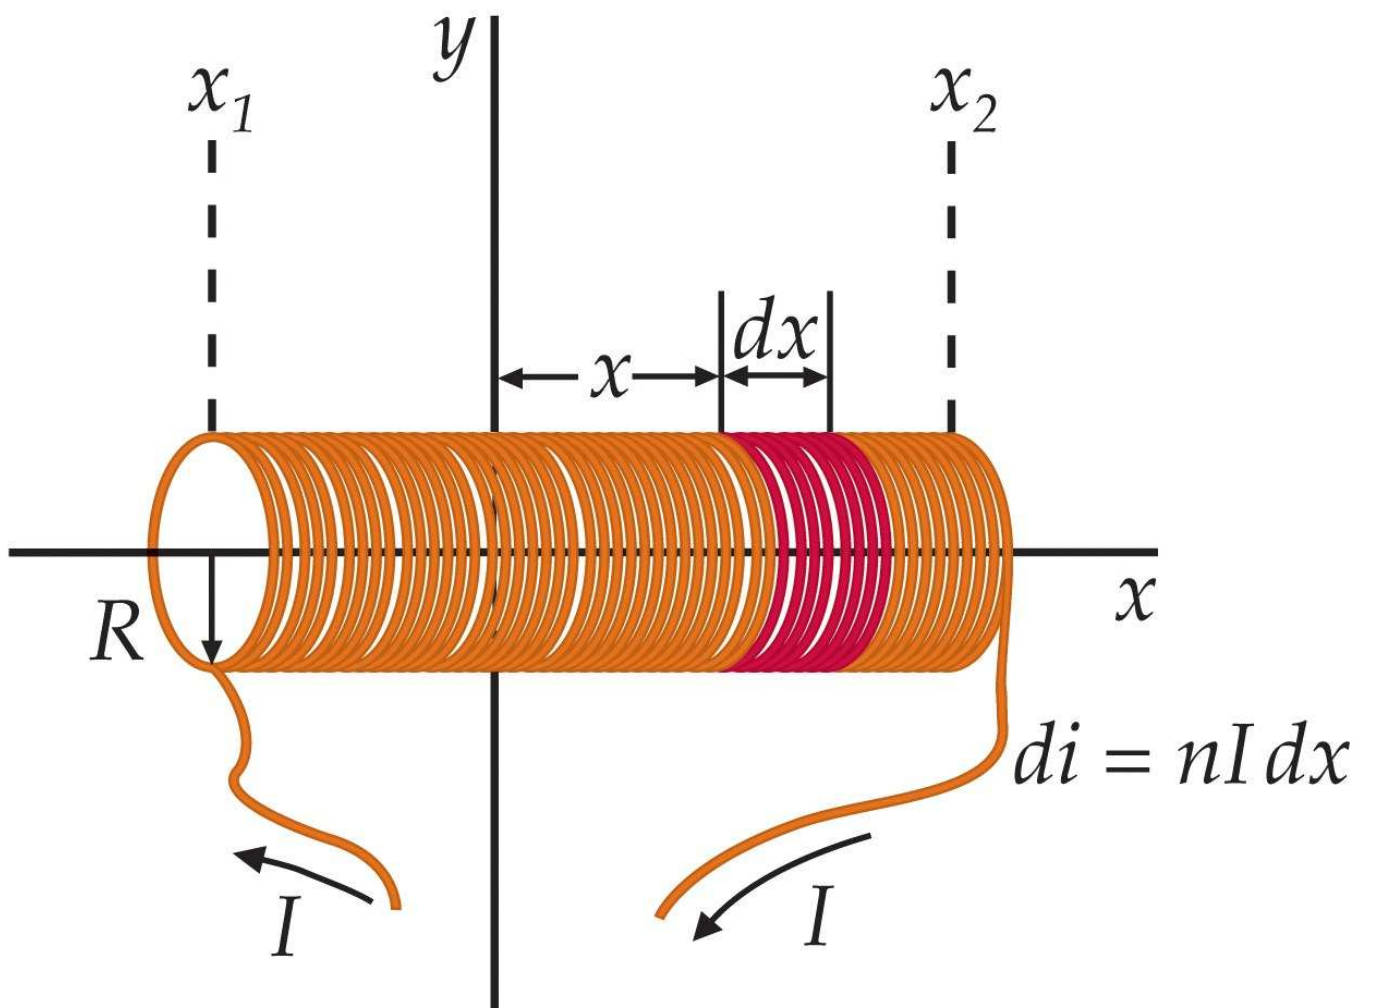
\includegraphics[width=300pt]{data/spule.png}
  \caption{Skizze einer Spule \cite{Spule}}
  \label{fig:spule}
\end{figure}

In der Skizze sind $x_1$ und $x_2$ die Anfangs- und Endpunkte der Wicklungen,
$\symup{d}x$ ist ein Wegelement zur Integration über die Spule. Durch dieses Wegelement
fließt ein kleiner Strom der Größe $\symup{d}i = n I \symup{d}x$. Dabei ist $n$
die Anzahl der Windungen pro Länge.
Der Betrag der magnetischen Flussdichte so einer Spule auf ihrer Symmetrieachse lässt sich durch
\eqref{eqn:biotsavart} zu
\begin{equation}
  B_x(x) = \frac{\mu_0 n I}{2} \left( \frac{x-x_1}{\sqrt{(x-x_1)^2+R^2}} - \frac{x-x_2}{\sqrt{(x-x_2)^2+R^2}} \right)
  \label{eqn:spuleungenaehert}
\end{equation}
berechnen. Hierbei wurden abgesehen von einem verschwindenden Querschnitt keinerlei Näherungen vorgenommen
\footnote{Die konkrete Berechnung wird hier nicht durchgeführt und kann in \cite{Spule} nachgelesen werden}.

Nähert man für eine Spule ihre Länge als deutlich größer gegenüber ihrem Durchmesser,
so ergibt sich näherungsweise für den Betrag der magnetischen Flussdichte durch Berechnung mit \eqref{eqn:biotsavart}
im Inneren der Spule
\begin{equation}
  B = \mu \frac{n}{l} I\,.
  \label{eqn:langespuleinnen}
\end{equation}
Dabei gilt für die Permeabilität $\mu = \mu_0 \mu_r$ mit der materialabhängigen
relativen Permeabilität $\mu_r$ und $l$ ist die Länge der Spule.
Die magnetische Flussdichte innerhalb der langen Spule ist ungefähr konstant, außerhalb
ist sie näherungsweise null.

Nahezu homogene Magnetfelder lassen sich mithilfe eines Helmholtz-Spulenpaars erzeugen, welches
in Abbildung \ref{fig:helmholtz} skizziert ist.

\begin{figure}
  \centering
  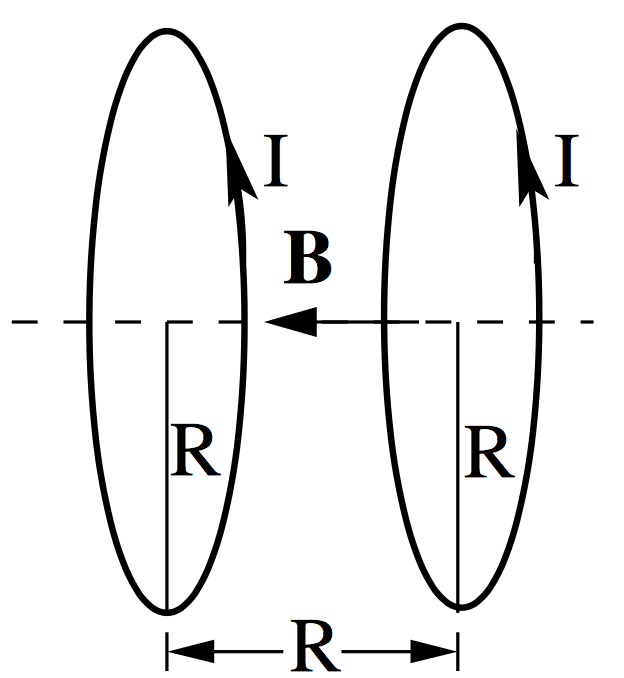
\includegraphics[width=150pt]{data/helmholtz.png}
  \caption{Skizze eines Helmholtzspulenpaars \cite{Versuchsanleitung}}
  \label{fig:helmholtz}
\end{figure}

Dieses besteht aus zwei in gleicher Richtung stromdurchflossenen Kreisspulen, die auf
auf einer gemeinsamen Achse aufgebaut werden. Ihr Abstand $d$ entspricht dem Spulenradius $R$.
Auf der Symmetrieachse zwischen den Spulen ist das Magnetfeld näherungsweise homogen. Dies lässt sich
ebenso mit dem Biot-Savartschen Gesetz \eqref{eqn:biotsavart} berechnen und ergibt sich nach \cite{Helmholtz} zu
\begin{equation}
  B_x(x) = \frac{\mu_0 i}{2 r} \left( \frac{1}{(\gamma^2+\gamma+5/4)^{3/2}} - \frac{1}{(\gamma^2-\gamma+5/4)^{3/2}} \right) \,.
  \label{eqn:helmholz}
\end{equation}
Dabei ist $i$ der Strom und $\gamma = x/r$ das Verhältnis aus dem Abstand auf der Spulenachse und dem Spulenradius $r$.

Hysterese bezeichnet die Eigenschaft eines Systems, dass sein Zustand von seiner Vergangenheit abhängt.
Diese Systeme sind nichtlinear und die charakteristischen Größen haben mehr als einen möglichen Wert für
einen Wert einer unabhängigen Variablen. Ein Beispiel für Systeme mit Hysterese sind
ferromagnetische Materialien. Eine sog. Hysterese- oder Magnetisierungskurve beschreibt
die Abhängigkeit der magnetischen Flussdichte $B$ des Stoffes, hervorgerufen durch
seine Magnetisierung, von dem äußeren magnetischen Feld $H$ und ist in Abbildung \ref{fig:hysteresetheorie}
skizziert.

\begin{figure}
  \centering
  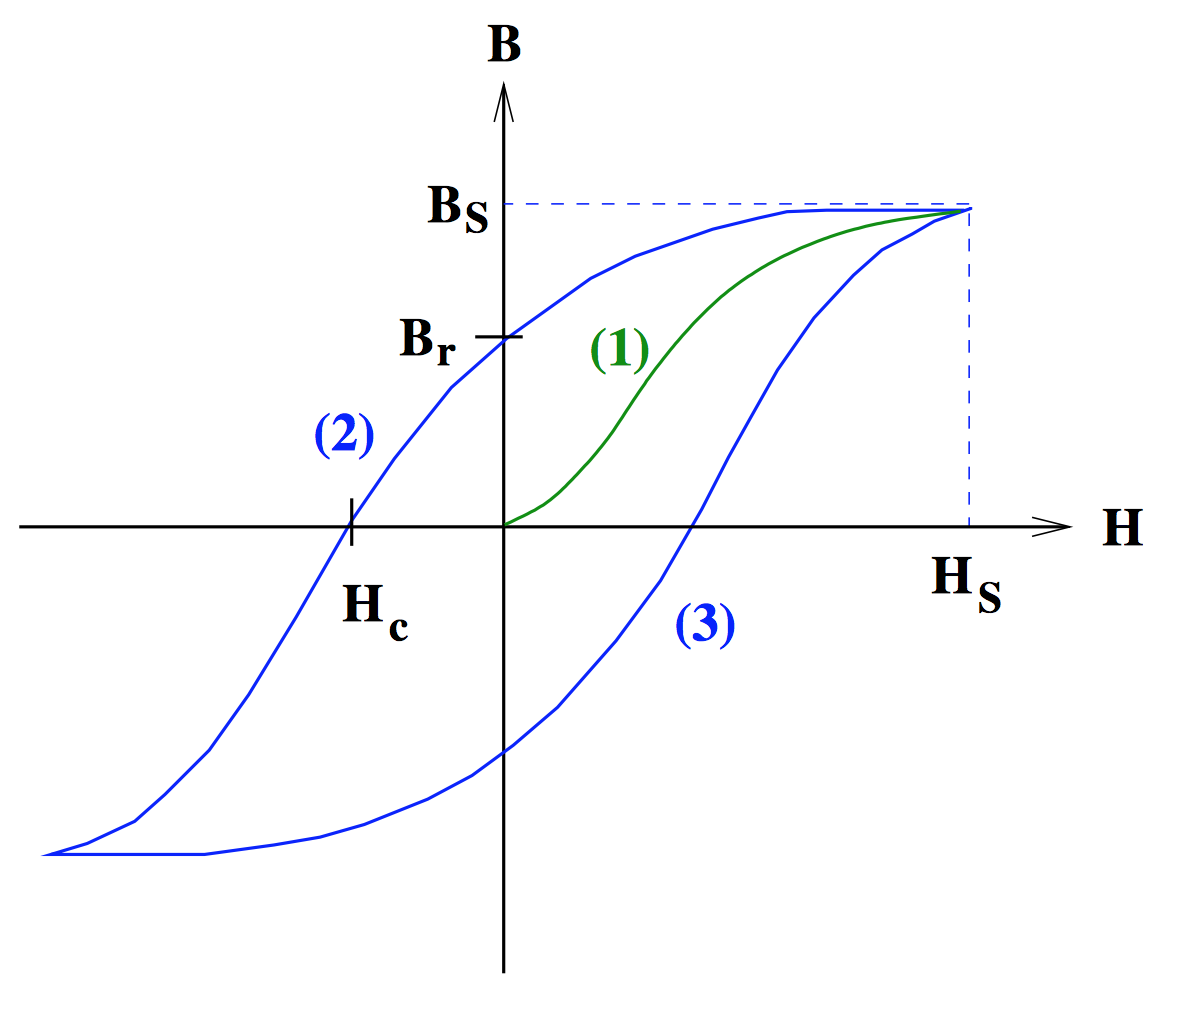
\includegraphics[width=300pt]{data/hysterese.png}
  \caption{Skizze einer Hysteresekurve \cite{Versuchsanleitung}}
  \label{fig:hysteresetheorie}
\end{figure}

Ist ein ferromagnetisches Material zunächst bei abgeschaltetem äußeren Feld unmagnetisiert,
erhält man bei langsamer Steigerung des äußeren Feldes eine Neukurve, in der Skizze
mit (1) bezeichnet und grün markiert.
Diese steigt bis auf den Sättigungswert $B_\text{s}$ an. Beim Verringern von $H$
sinkt die Magnetisierung (Kurvenverlauf (2)), bis bei vollständig abgeschaltetem Feld die Remanenz übrig
bleibt. Diese übrig gebliebene magnetische Flussdichte kann durch die Koerzitivkraft
$H_\text{c}$ vollständig aufgehoben werden, bis der Sättigungswert schlussendlich wieder
im dritten Quadranten des Koordinatensystems erreicht wird. Die Kurve schließt sich
im gleichen Verlauf (Kurvenverlauf (3)) wieder bis zur positiven Sättigung und ist somit symmetrisch zum Ursprung.
Wird ein äußeres Magnetfeld $H$ durch einen Strom $I$ erzeugt, ergibt auch das Auftragen
von $B$ gegen $I$ eine Hysteresekurve, da das äußere Feld proportional zur Stromstärke ist.

Die Messung magnetischer Felder geschieht in der Regel mithilfe einer Hall-Sonde.
In ihr befindet sich ein Metallplättchen, das von einem konstanten Strom durchflossen wird.
Ein äußeres magnetisches Feld übt Kraft auf die bewegten elektrischen Ladungen aus
und trennt sie. Dies erzeugt eine Spannung und wird auch Hall-Effekt genannt.
Diese Spannung ist ein Maß für die Stärke der Flussdichte des äußeren magnetischen Feldes, welche
dann abgelesen werden kann. Je nach zu untersuchender Geometrie sind longitudinale und transversale Hall-Sonden
zu verwenden.
